\documentclass[12pt,a4paper]{article}

\usepackage[utf8]{inputenc}
\usepackage[T2A]{fontenc}
\usepackage[ukrainian]{babel}

\usepackage{geometry}
\geometry{left=2cm,right=2cm,top=2cm,bottom=2cm}

\usepackage{graphicx}
\usepackage{array,multirow}
\usepackage{booktabs}
\usepackage{caption}
\usepackage{subcaption}
\renewcommand{\thetable}{№\arabic{table}}
\captionsetup[subfigure]{labelformat=simple,labelsep=space}

\usepackage{amsmath}
\usepackage{pdflscape}
\usepackage{xcolor}

\usepackage{hyperref}

\renewcommand\thesubfigure{(\alph{subfigure})}

\begin{document}

    \begin{titlepage}

        % Картинка шапки (по центру, з відступом від верху)
        \begin{center}
\includegraphics[width=0.7\textwidth]{../../../TITLES/letterhead.png}\end{center}

        \begin{center}
            \large Національний технічний університет України\\
            «Київський політехнічний інститут імені Ігоря Сікорського»\\[1em]
            Факультет інформатики та обчислювальної техніки\\
            Кафедра обчислювальної техніки
        \end{center}

        \vfill

        \begin{center}
            \textbf{\LARGE Практична електроніка}\\[2em]
            \textbf{\Large Лабораторна робота №4}\\[1em]
            «Дослідження імпульсних тригерів, аналогових компараторів та схем формування рівнів»
        \end{center}

        \vfill

        \begin{flushright}
            Виконав: студент 2 курсу ФІОТ, гр. ІО-41\\
            \textit{Давидчук А.~М.}\\[1em]
            Перевірив: \textit{Гайдай А.~Р.}
        \end{flushright}

        \vfill

        \begin{center}Київ --- 2025\end{center}

    \end{titlepage}

    % Основний документ:

    \setlength{\parindent}{0em}

    \textbf{\underline{Тема:}} «Дослідження імпульсних тригерів, аналогових компараторів та схем формування рівнів».

    \vspace{1em}

    \textbf{\underline{Мета:}} Дослідити принцип дії, основні властивості та характеристики
    імпульсних тригерів (ІТ), аналогових компараторів (АК) та схем формування рівнів
    (СФР). Ознайомитись із основними параметрами цих пристроїв та областю їх
    застосування.

    \begin{center} \textbf{\Large Практична частина} \end{center}

    Мій номер залікової книги 6, звідси $N = 6$.

    \begin{center} \textbf{\large Аналіз схеми №1: АК для порівняння однополярних напруг} \end{center}

    \setlength{\parindent}{1.5em}

    Нижче наведено схему АК для порівняння однополярних напруг, яку зібрано у середовищі MicroCap:

    \begin{figure}[h!]

        \renewcommand{\thefigure}{\arabic{figure}} % робимо "3.1", "3.2" і т.д.

        \centering
        \includegraphics[width=0.7\textwidth]{scheme1.pdf}
        \caption{Схема АК для порівняння однополярних напруг}

    \end{figure}

    \newpage

    На рис. 2 наведена передатна характеристика та часові діаграми роботи АК для порівняння однополярних напруг, схему якого наведено на рис. 1.
    На рис. 2 зображено часові діаграми роботи однополярного АК, який порівнює дві додатні напруги, одна з яких є еталонною, яка не змінюється і дорівнює
    5В, а друга змінюється за трикутним законом:

    \begin{figure}[h!]
        \centering

        \begin{subfigure}{1.0\textwidth}
            \centering
            
\includegraphics[width=\linewidth]{graph1-2.png}
            \caption{Передатна характеристика}
        \end{subfigure}\vfill
        \begin{subfigure}{1.0\textwidth}
            \centering
            
\includegraphics[width=\linewidth]{graph1-1.png}
            \caption{Часові діаграми}
        \end{subfigure}

        \caption{\centering Передатна характеристика та часові діаграми роботи АК для порівняння однополярних напруг}
    \end{figure}

    Лінія, яка характеризує вихідну напругу, лежить в межах:
    \[
    -U_{\text{нас}} \le U_{\text{вих}} \le +U_{\text{нас}}.
    \]

    Її невеликий нахил та невідповідність $-U_{\text{нас}}$ й $+U_{\text{нас}}$ на характеристиці пояснюється наявністю затримки між досягненням $U_{\text{вих}}$ значення еталонної напруги та зміною вихідної напруги.

    На схемі АК, щоб врівноважити струми при $U_{\text{вх}}=0$ і $U_{\text{оп}}=0$ повинно виконуватись співвідношення: $R_1=R_2$. Робота цієї схеми характеризується величиною напруги $U_{\text{оп}}$ і точками, в яких $U_{\text{вх}}=U_{\text{оп}}$. Тобто в початковий момент часу, крім напруг живлення на підсилювач подаються напруги $U_{\text{вх}}=0$ і $U_{\text{оп}}=5\text{В}$. Оскільки потенціал на вході, який не інвертує, та дорівнює $U_{\text{оп}}$, більш додатний, ніж на вході, який інвертує ($U_{\text{вх}}$), то на виході отримаємо $+U_{\text{нас}}$. 

    В момент часу $t_1$, коли потенціал $U_{\text{вх}}$ стає більш додатним, ніж $U_{\text{оп}}$, \, то відбувається перемикання компаратора і на виході отримаємо $-U_{\text{нас}}$. Коли вихідний сигнал стає менш додатним, ніж $U_{\text{оп}}$ (момент часу $t_2$), на виході знову отримаємо $+U_{\text{нас}}$. 

    Для побудови графіків будемо обирати час аналізу залежно від часу подачі імпульсів. Наприклад, на даному графіку обрано час $60$ мілісекунд.

    \begin{center} \textbf{\large Аналіз схеми №2: АК для порівняння однополярних напруг за умови наявності завад} \end{center}

    Нижче наведено схему АК для порівняння однополярних напруг за умови наявності завад, яку зібрано у середовищі MicroCap:

    \begin{figure}[h!]

        \renewcommand{\thefigure}{\arabic{figure}} % робимо "3.1", "3.2" і т.д.

        \centering
        \includegraphics[width=0.7\textwidth]{scheme2.pdf}
        \caption{Схема АК для порівняння однополярних напруг за умови наявності завад}

    \end{figure}

    \newpage

    На рис. 4 наведена передатна характеристика та часові діаграми роботи АК, схему якого наведено на рис. 3.

    В даному випадку розглядається синусоїдальна завада значно вищої частоти, ніж $U_{\text{вх}}$. Завада накладається на вхідний трикутний сигнал.

    \begin{figure}[h!]
        \centering

        \begin{subfigure}{1.0\textwidth}
            \centering
            
\includegraphics[width=\linewidth]{graph2-2.png}
            \caption{Передатна характеристика}
        \end{subfigure}\vfill
        \begin{subfigure}{1.0\textwidth}
            \centering
            
\includegraphics[width=\linewidth]{graph2-1.png}
            \caption{Часові діаграми}
        \end{subfigure}

        \caption{\centering Передатна характеристика та часові діаграми роботи АК, схему якого наведено на рис. 3}
    \end{figure}

    Через наявність завад у разі повільної зміни вхідної напруги можемо спостерігати швидку та часту зміну вихідної напруги (так званий «брязкіт»), що приводить до помилкових спрацьовувань логічних лічильних схем, які підраховують кількість спрацьовувань компаратора.

    Щоб врівноважити струми за $U_{\text{вх}}=0$ та $U_{\text{оп}}=0$ повинно виконуватись співвідношення: $R_1=R_2$.

    На вході, який інвертує, відбувається підсумовування сигналів від джерел $V_4$ та $V_5$, тобто поки ця сума менше $V_3$, на виході отримуємо: $+U_{\text{нас}}$. Коли ця сума стає більшою за $V_3$, на виході отримуємо: $-U_{\text{нас}}$. Через наявність завад з'являються помилки спрацьовування компаратора.

    Для виправлення цього використовують гістерезис (у схему вводять додатний зворотний зв'язок, ДЗЗ), під час якого замість одного значення, за яким здійснюється спрацьовування схеми, вводять певний діапазон. Це погіршує точність роботи схеми, тобто вона спрацьовує пізніше, але ми позбавляємось «брязкоту».

    \begin{center} \textbf{\large Аналіз схеми №3: АК з ДЗЗ для порівняння однополярних напруг за умови наявності завад (регенеративний АК) } \end{center}

    Нижче наведено схему АК з ДЗЗ для порівняння однополярних напруг за умови наявності завад (регенеративний АК), яку зібрано у середовищі MicroCap:

    \begin{figure}[h!]

        \renewcommand{\thefigure}{\arabic{figure}} % робимо "3.1", "3.2" і т.д.

        \centering
        \includegraphics[width=0.7\textwidth]{scheme3.pdf}
        \caption{\centering Схема регенеративного АК}

    \end{figure}

    На рис. 6 представлено часові діаграми роботи АК, схему якого наведено на рис. 5:

    \begin{figure}[h!]
        \centering
        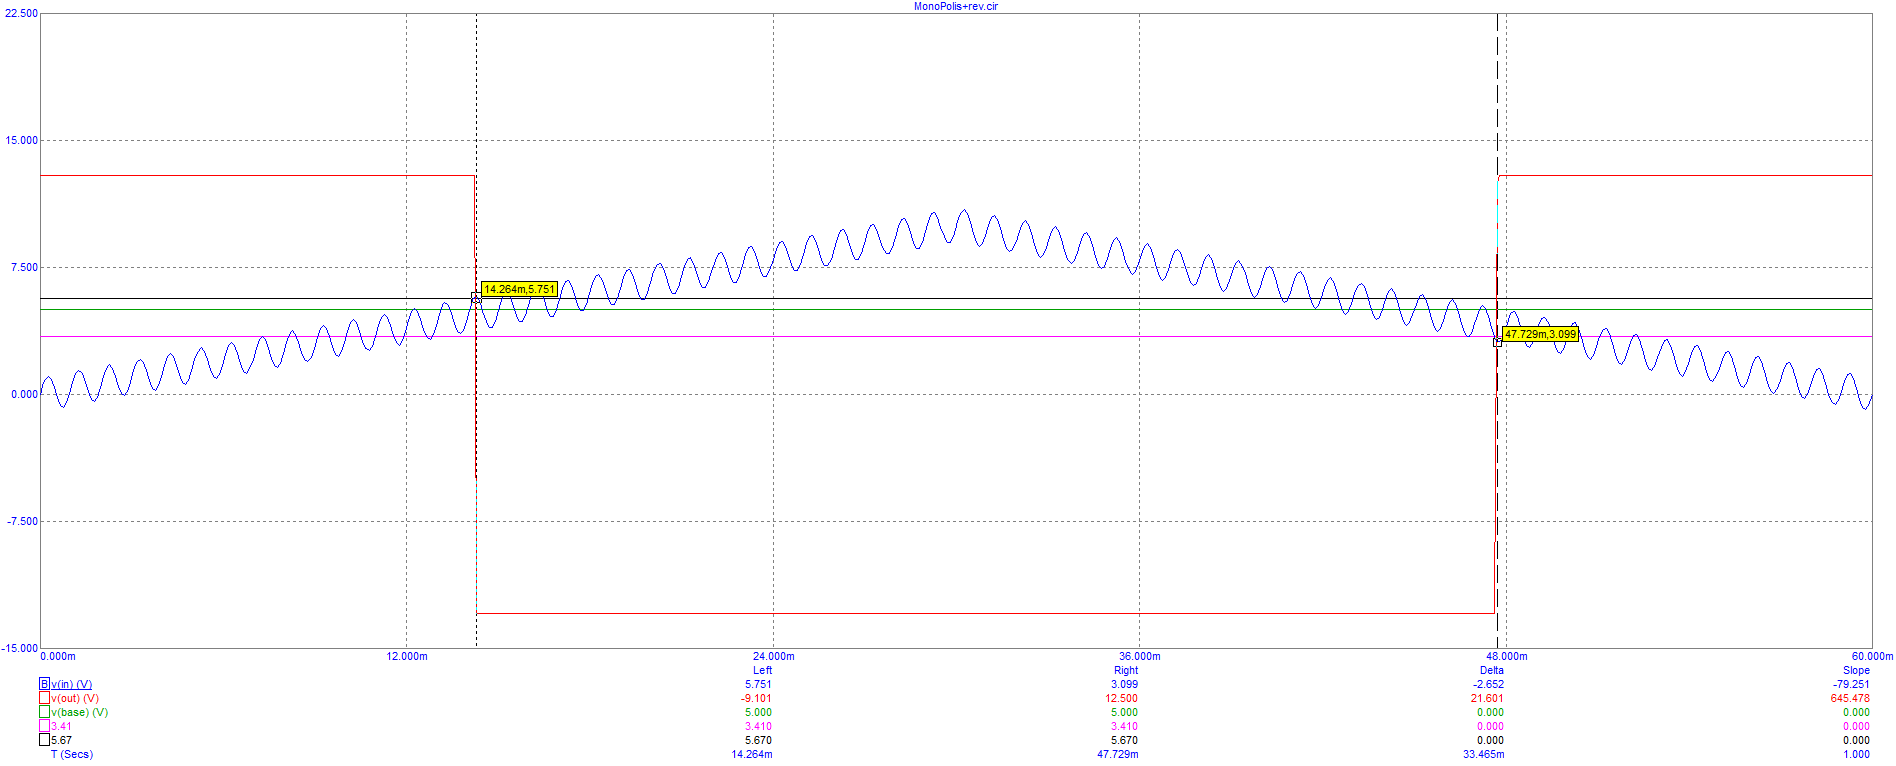
\includegraphics[width=\linewidth]{graph3.png}
        \caption{Часові діаграми роботи регенеративного АК}
    \end{figure}

    Як видно з графіка, схема спрацьовує пізніше, але позбавляється зайвих спрацьовувань.

    \[
    \text{Якщо } U_{\text{вих}} = +U_{\text{нас}}, \quad
    U_{H1} \approx 5{,}751~\text{В}.
    \]

    \[
    \text{Якщо } U_{\text{вих}} = -U_{\text{нас}}, \quad
    U_{H2} \approx 3{,}099~\text{В}.
    \]

    \[
    \text{Напруга гістерезису } \Delta U_{\text{Г}}
    = U_{H1} - U_{H2}
    = 5{,}751 - 3{,}099
    = 2{,}652~\text{В}.
    \]

    Якщо рівень завади \(U_{\text{завд}}\) менший, ніж \(\Delta U_{\text{Г}}\),
    то у схемі не відбувається хибних спрацьовувань; точність порівняння дещо
    погіршується, зате компаратор спрацьовує стабільніше.

    \begin{center} \textbf{\large Аналіз схеми №4: АК для порівняння різнополярних напруг} \end{center}

    Нижче наведено схему АК для порівняння різнополярних напруг, яку зібрано
у середовищі MicroCap:

    \begin{figure}[h!]

        \renewcommand{\thefigure}{\arabic{figure}} % робимо "3.1", "3.2" і т.д.

        \centering
        \includegraphics[width=0.7\textwidth]{scheme4.pdf}
        \caption{\centering Схема АК для порівняння різнополярних напруг}

    \end{figure}

    \newpage

    На рис. 8 наведена передатна характеристика та часові діаграми
роботи АК для порівняння різнополярних напруг, схему якого наведено на
рис. 7:

    \begin{figure}[h!]
        \centering

        \begin{subfigure}{1.0\textwidth}
            \centering
            
\includegraphics[width=\linewidth]{graph4-2.png}
            \caption{Передатна характеристика}
        \end{subfigure}\vfill
        \begin{subfigure}{1.0\textwidth}
            \centering
            
\includegraphics[width=\linewidth]{graph4-1.png}
            \caption{Часові діаграми}
        \end{subfigure}

        \caption{\centering Часові діаграми роботи та передатна характеристика АК для порівняння
        різнополярних імпульсів, схему якого наведено на рис. 7
        }
    \end{figure}

    Відмінність часових характеристик різнополярного АК без завад від
однополярного АК без завад — наявність від’ємної еталонної напруги
$5\,\text{В}$ та додатної вхідної трикутної напруги, які порівнюються
на вході, який інвертує. До моменту $t_1$ потенціал входу, який
інвертує, від’ємний, і на виході: $+\!U_{\text{нас}}$. Після моменту
$t_1$ потенціал цього входу стає додатним, і схема переключається у
$-\!U_{\text{нас}}$.

    \newpage

    \begin{center} \textbf{\large Аналіз схеми №5: ТШ на базі ІМС ОП з пам’яттю} \end{center}

    Нижче наведено схему ТШ на базі ІМС ОП з пам’яттю, яку зібрано у
середовищі MicroCap:

    \begin{figure}[h!]

        \renewcommand{\thefigure}{\arabic{figure}} % робимо "3.1", "3.2" і т.д.

        \centering
        \includegraphics[width=0.7\textwidth]{scheme5.pdf}
        \caption{\centering Схема ТШ на базі ІМС ОП з пам’яттю}

    \end{figure}

    На рис.~10 наведена передатна характеристика та часові діаграми
    роботи ТШ на базі ІМС ОП з пам’яттю, схему якого наведено на
    рис.~9.

    Згідно з передатною характеристикою, за $U_{\text{вх}} = 0$ на виході
    схеми може випадково з’явитися напруга $+U_{\text{нас}}$ або
    $-U_{\text{нас}}$. Так, на рис.~10 (вгорі) це напруга $-U_{\text{нас}}$,
    тобто схема умовно спрацювала. Коли від’ємна напруга дорівнює $-0{,}62\,\text{В}$,
    схема «відпустить», та знову спрацює, якщо $U_{\text{вх}} = +0{,}62\,\text{В}$ і т.~д.
    За $U_{\text{вх}} = 0$ схема не змінює (запам’ятовує) свій попередній стан.

    \newpage

    На рис.~10 (вгорі) зображено реакцію ТШ на базі ІМС ОП з пам’яттю на
    синусоїдальний сигнал. ТШ кожний раз після спрацьовування запам’ятовує
    останній стан за $U_{\text{вх}} = 0$ і починає роботу з нього, що свідчить
    про наявність пам’яті.

    \begin{figure}[h!]
        \centering

        \begin{subfigure}{0.7\textwidth}
            \centering
            
\includegraphics[width=\linewidth]{graph5-1.png}
            \caption{Часові діаграми}
        \end{subfigure}\vfill
        \begin{subfigure}{0.7\textwidth}
            \centering
            
\includegraphics[width=\linewidth]{graph5-2.png}
            \caption{Передатна характеристика}
        \end{subfigure}

        \caption{\centering
        Часові діаграми роботи та передатна характеристика ТШ на базі ІМС ОП з пам’яттю
        }
    \end{figure}

    \[
    U_{\text{спр}} = 
    \frac{U_{\text{нас}} \cdot R_2}{R_2 + R_4}
    - 
    \frac{U_{\text{нас}}}{K_{U,\text{ІМС ОП}}}
    = 0{,}62\,\text{В},
    \]

    \[
    U_{\text{відп}} = 
    -\frac{U_{\text{нас}} \cdot R_2}{R_2 + R_4}
    + 
    \frac{|U_{\text{нас}}|}{K_{U,\text{ІМС ОП}}}
    = -0{,}62\,\text{В}.
    \]

    На рис.~10 (вгорі) нанесено лінії, що відповідають напругам:
    $U_{\text{спр}} = 0{,}62\,\text{В}$, 
    $U_{\text{відп}} = -0{,}62\,\text{В}$.
    Аналіз діаграм показує, що результат збігається з наведеними вище розрахунками в межах допустимої похибки.

    \begin{center} \textbf{\large Аналіз схеми №6: ТШ на базі ІМС ОП без пам’яті } \end{center}

    Нижче наведено схему ТШ на базі ІМС ОП без пам’яті, яку зібрано у
середовищі MicroCap:

    \begin{figure}[h!]

        \renewcommand{\thefigure}{\arabic{figure}} % робимо "3.1", "3.2" і т.д.

        \centering
        \includegraphics[width=0.7\textwidth]{scheme6.pdf}
        \caption{\centering Схема ТШ на базі ІМС ОП без пам’яті }
    \end{figure}

    На рис.~12 наведена передатна характеристика та часові діаграми
    роботи ТШ на базі ІМС ОП без пам’яті, схему якого наведено на
    рис.~11.

    Згідно з передатною характеристикою, за $U_{\text{вх}} = 0$ на виході
    з’являється напруга $+U_{\text{нас}}$. Коли $U_{\text{вх}} > U_{\text{спр}}$,
    схема переключається у $-U_{\text{нас}}$. За $U_{\text{вх}} < U_{\text{відп}}$
    схема повертається у початковий стан. Тобто схема не має пам’яті й працює
    як пороговий пристрій.

    \newpage

    \begin{figure}[h!]
        \centering

        \begin{subfigure}{0.95\textwidth}
            \centering
            
\includegraphics[width=\linewidth]{graph6-1.png}
            \caption{Часові діаграми}
        \end{subfigure}\vfill
        \begin{subfigure}{0.95\textwidth}
            \centering
            
\includegraphics[width=\linewidth]{graph6-2.png}
            \caption{Передатна характеристика}
        \end{subfigure}

        \caption{\centering
        Часові діаграми роботи та передатна характеристика ТШ на базі ІМС ОП без пам’яті 
        }
    \end{figure}

    \newpage

    На рис.~12 (вгорі) зображено реакцію ТШ на базі ІМС ОП без пам’яті на
    послідовність трикутних імпульсів. ТШ кожен раз після спрацьовування, коли
    рівень вхідної напруги стає меншим за $U_{\text{відп}}$, повертається у
    початковий стан, що свідчить про відсутність пам’яті.

    Використовуючи принцип суперпозиції, одержимо:
    \[
    U_{H1} =
    \frac{U_{\text{оп}} \cdot R_3}{R_2 + R_4} +
    \frac{U_{\text{нас}} \cdot R_2}{R_2 + R_4}
    = U_{\text{спр}}.
    \]

    \[
    U_{\text{спр}} =
    5 \cdot \frac{10}{0{,}5 + 10} +
    13 \cdot \frac{0{,}5}{0{,}5 + 10}
    = 4{,}76 + 0{,}61 = 5{,}38~\text{В}.
    \]

    \[
    U_{H2} =
    \frac{U_{\text{оп}} \cdot R_3}{R_2 + R_4} -
    \frac{U_{\text{нас}} \cdot R_2}{R_2 + R_4}
    = U_{\text{відп}}.
    \]

    \[
    U_{\text{відп}} = 4{,}76 - 0{,}61 = 4{,}14~\text{В}.
    \]

    \begin{center} \textbf{\large Аналіз схеми №7: Формувач рівнів} \end{center}

    Нижче наведено схему формувача рівнів, яку зібрано у середовищі
MicroCap:

    \begin{figure}[h!]

        \renewcommand{\thefigure}{\arabic{figure}} % робимо "3.1", "3.2" і т.д.

        \centering
        \includegraphics[width=0.7\textwidth]{scheme7.pdf}
        \caption{\centering Схема пристрою формувача рівнів}
    \end{figure}

    На рис. 14 наведено часові діаграми роботи схеми формувача рівнів.

    \newpage

    \begin{figure}[h!]
        \centering
        
\includegraphics[width=\linewidth]{graph7.png}
        \caption{Часові діаграми роботи схеми формувача рівнів, яку наведено на рис. 13}
    \end{figure}

    Цей пристрій перетворює:
    \begin{itemize}
        \item напругу $U_{\text{вх}} = +U_{\text{нас}}$ у напругу 
        $U_{\text{вих}} = U^{1} = U_{\text{VD2.пр}} + E_{\text{ЕТ}}; \quad
        E_{\text{ЕТ}} = V1;$

        \[
        U_{\text{вих}} = 0{,}6 + 4 = 4{,}6~\text{В};
        \]

        \item напругу $U_{\text{вх}} = -U_{\text{нас}}$ у напругу 
        $U_{\text{вих}} = U^{0} = I_{\text{КО.VD2}} \cdot R_{H},$
        
        де $I_{\text{КО.VD2}}$ — зворотний струм насичення закритого діода VD2.

        \[
        U_{\text{вих}} = 0{,}6 \cdot 10^{-6} \cdot 10^{5} = 0{,}06~\text{В}.
        \]
    \end{itemize}

    \begin{center} \textbf{\large Аналіз схеми №8: Асинхронний RS-тригер із зовнішнім зміщенням} \end{center}

    Нижче наведено схему асинхронного RS-тригера із зовнішнім зміщенням, яку
зібрано у середовищі MicroCap:

    \begin{figure}[h!]

        \renewcommand{\thefigure}{\arabic{figure}} % робимо "3.1", "3.2" і т.д.

        \centering
        \includegraphics[width=0.7\textwidth]{scheme8.pdf}
        \caption{\centering Асинхронний RS-тригер із зовнішнім зміщенням}

    \end{figure}

    На рис. 16 наведено часові діаграми роботи асинхронного RS-тригера із зовнішнім зміщенням:

    \begin{figure}[h!]
        \centering
        
\includegraphics[width=\linewidth]{graph8.png}
        \caption{Часові діаграми роботи асинхронного RS–тригера із зовнішнім зміщенням}
    \end{figure}

    Як добре видно на часовій діаграмі, за $S = 0$ та $R = 0$ схема займає
    стан нестійкої невизначеності; за $S = 1, R = 0$ — стан $Q = 1$,
    $\overline{Q} = 0$, тригер перемкнувся в одиницю; за $S = 0, R = 1$ —
    $Q = 0$, $\overline{Q} = 1$, тригер перемкнувся в нуль; за
    $S = 1, R = 1$ (забороненій комбінації) — виходи тригера інвертуються на
    основі попередніх значень, що є похибкою моделювання.

    \newpage

    \begin{center} \textbf{\large Аналіз схеми №9: Асинхронний RS-тригер із зовнішнім зміщенням} \end{center}

    Нижче наведено схему асинхронного RS-тригера із зовнішнім зміщенням, яку
зібрано у середовищі MicroCap:

    \begin{figure}[h!]

        \renewcommand{\thefigure}{\arabic{figure}} % робимо "3.1", "3.2" і т.д.

        \centering
        \includegraphics[width=0.7\textwidth]{scheme9.pdf}
        \caption{\centering Тригер з лічильним входом}

    \end{figure}

    Як видно з рис. 18, тригер змінює свій стан на протилежний за кожним
від’ємним імпульсом на вході Т, який лічить:

    \begin{figure}[h!]
        \centering
        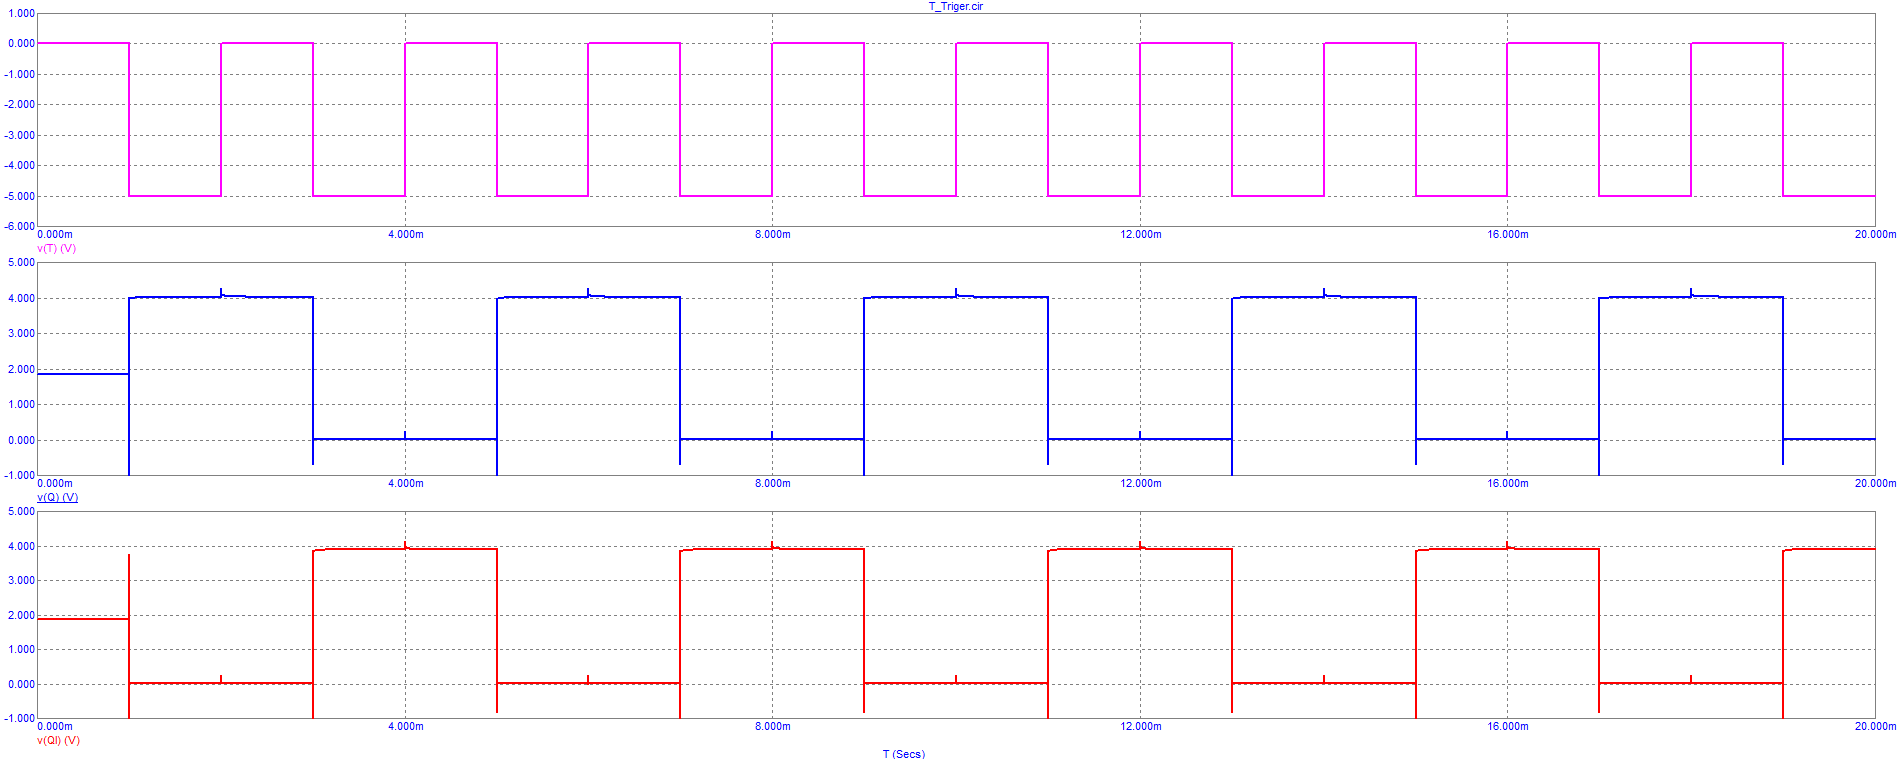
\includegraphics[width=\linewidth]{graph9.png}
        \caption{Часові діаграми тригера з лічильним входом}
    \end{figure}

    \noindent
    \textbf{\underline{Висновок:}} 
    Під час лабораторної роботи досліджено роботу аналогових компараторів, тригерів Шмітта та формувача рівнів у середовищі MicroCap.  
Встановлено, що додатний зворотний зв’язок (гістерезис) підвищує завадостійкість компараторів, зменшуючи кількість хибних спрацьовувань.  

Тригери Шмітта з пам’яттю зберігають попередній стан, а без пам’яті працюють як порогові пристрої.  
Формувач рівнів забезпечує потрібні логічні рівні сигналів.

Результати моделювання підтвердили теоретичні очікування, невеликі розбіжності пов’ язані з інерційністю операційного підсилювача.

\end{document}